\section{Application Profiling}

\begin{frame}
  \frametitle{Profiling}
  \begin{itemize}
    \item Profiling is the act of gathering data from a program execution in
          order to analyze them and then optimize or fix performance issues.
    \item Profiling is achieved by using programs that insert instrumentation
          in the code or leverage kernel/userspace mechanisms.
    \begin{itemize}
      \item Profiling function calls and count of calls allow to optimize
            performances.
      \item Profiling processor usage allows to optimize performances and
            reduce power usage.
      \item Profiling memory usage allows to optimize memory consumption.
    \end{itemize}
    \item After profiling, the data set must be analyzed to identify potential
          improvements (and not the reverse !).
  \end{itemize}
\end{frame}

\begin{frame}
  \frametitle{Performance issues}
  \begin{center}
    \vspace{0.2cm}
    \em{"Premature optimization is the root of all evil", Donald Knuth}
  \end{center}
  \begin{itemize}
    \item Profiling is often useful to identify and fix performance issues.
    \item Performances can be affected by memory usage, IOs overload, or
          CPU usage.
    \item Gathering profiling data before trying to fix performance issues is
          needed to do the correct choices.
    \item Profiling is often guided by a first coarse-grained analysis using
          some classic tools.
    \item Once the class of problems has been identified, a fine grain
          profiling analysis can be done.
  \end{itemize}
\end{frame}

\begin{frame}
  \frametitle{Profiling metrics}
  \center 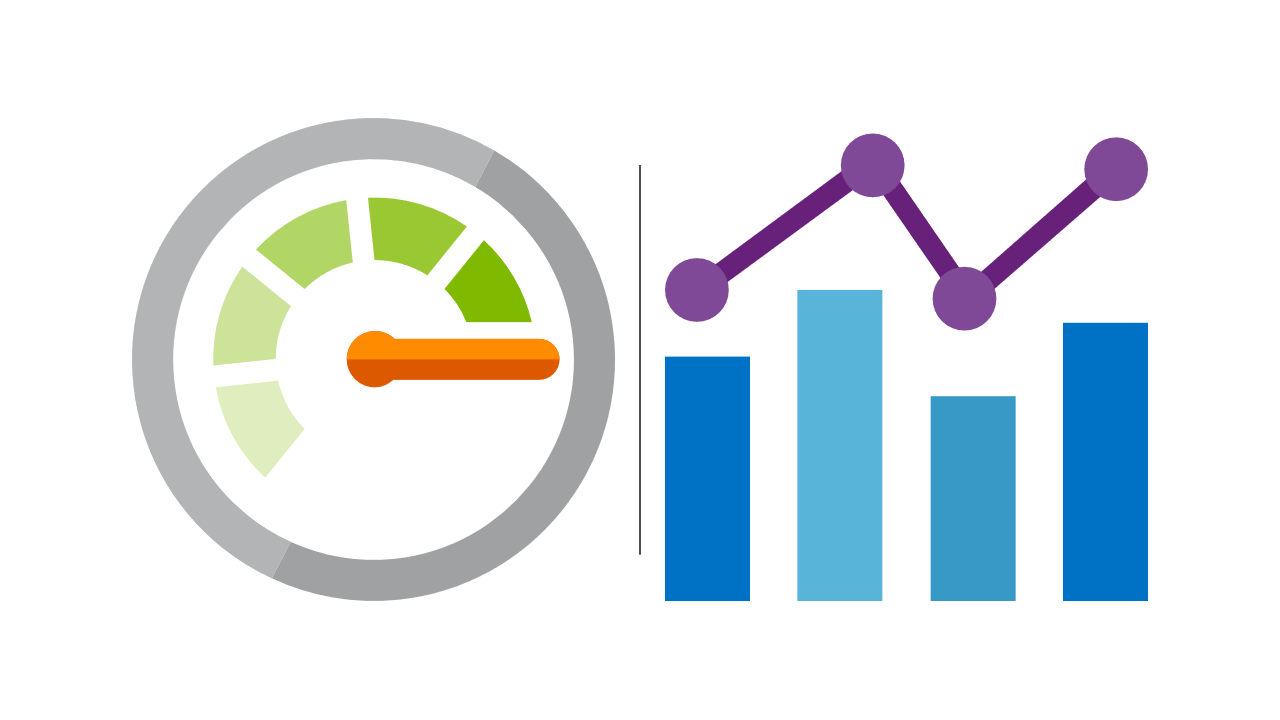
\includegraphics[width=0.3\textwidth]{../slides/debugging-application-profiling/metrics.png}
  \begin{itemize}
    \item Multiple tools allows to profile various metrics.
    \item Memory usage with {\em Massif}, \code{heaptrack} or memusage.
    \item Function calls using {\em perf} and callgrind.
    \item CPU hardware usage (Cache, MMU, etc) using {\em perf}.
    \item Profiling data can include both the user space application and kernel.
  \end{itemize}
\end{frame}

\begin{frame}
  \frametitle{Memory profiling}
  \begin{itemize}
    \item Profiling memory usage (heap/stack) in a application is useful for
          optimization.
    \item Allocating too much memory can lead to system memory exhaustion.
    \item Allocating/freeing memory too much can lead to the kernel spending a
          considerable amount of time in \code{clear_page}.
    \item Reducing application memory footprint can allow optimizing cache usage
          as well as page miss.
  \end{itemize}
\end{frame}

\begin{frame}[fragile]
  \frametitle{Massif usage}
  \begin{itemize}
    \item {\em Massif} is a tool provided by {\em valgrind} which allows to profile
          heap usage during the program execution (user-space only).
    \item Works by making snapshots at allocations.
  \end{itemize}
  \begin{block}{}
    \begin{minted}[fontsize=\small]{console}
$ valgrind --tool=massif --time-unit=B program
    \end{minted}
  \end{block}
  \begin{itemize}
    \item Once executed, a {\em massif.out.<pid>} file will be generated in the
          current directory
    \item \code{ms_print} tool can then be used to display a graph of heap allocation
  \end{itemize}

  \begin{block}{}
    \begin{minted}[fontsize=\small]{console}
$ ms_print massif.out.275099
    \end{minted}
  \end{block}
  \begin{itemize}
    \item \code{@}: Detailed snapshot
    \item \code{#}: Peak allocation
  \end{itemize}
\end{frame}

\begin{frame}[fragile]
  \frametitle{Massif report}
  \begin{block}{}
    \begin{minted}[fontsize=\tiny]{console}
KB
547.0^                                               # :: : :@ : :: :         
      |                                             @:#:::::::@::::::::@       
      |                                           ::@:#:::::::@::::::::@::     
      |                                        :::::@:#:::::::@::::::::@:::::  
      |                                      :::::::@:#:::::::@::::::::@:::::::
      |                                      :::::::@:#:::::::@::::::::@:::::::
      |                                      :::::::@:#:::::::@::::::::@:::::::
      |                                      :::::::@:#:::::::@::::::::@:::::::
      |                              @@@@@@@@:::::::@:#:::::::@::::::::@:::::::
      |                              @       :::::::@:#:::::::@::::::::@:::::::
      |                              @       :::::::@:#:::::::@::::::::@:::::::
      |                       :::::::@       :::::::@:#:::::::@::::::::@:::::::
      |                       :      @       :::::::@:#:::::::@::::::::@:::::::
      |                 :::::::      @       :::::::@:#:::::::@::::::::@:::::::
      |                 :     :      @       :::::::@:#:::::::@::::::::@:::::::
      |            ::::::     :      @       :::::::@:#:::::::@::::::::@:::::::
      |            :    :     :      @       :::::::@:#:::::::@::::::::@:::::::
      |        :::::    :     :      @       :::::::@:#:::::::@::::::::@:::::::
      |     ::::   :    :     :      @       :::::::@:#:::::::@::::::::@:::::::
      |  ::::  :   :    :     :      @       :::::::@:#:::::::@::::::::@:::::::
    0 +----------------------------------------------------------------------->KB
      0                                                                   830.5

Number of snapshots: 52
  Detailed snapshots: [9, 19, 22 (peak), 32, 42]
    \end{minted}
  \end{block}
\end{frame}

\begin{frame}[fragile]
  \frametitle{heaptrack usage}
  \begin{itemize}
    \item {\em heaptrack} is a heap memory profiler for Linux.
    \begin{itemize}
      \item Works with \code{LD_PRELOAD} library.
    \end{itemize}
    \item Finer tracking than with Massif and visualizing tool is more advanced.
    \begin{itemize}
      \item Each allocation is associated to a stacktrace
      \item Allows finding memory leaks, allocation hotspots and
            temporary allocations.
    \end{itemize}
    \item Results can be seen using GUI (\code{heaptrack_gui} or CLI tool
          (\code{heaptrack_print}).
    \item \url{https://github.com/KDE/heaptrack}
  \end{itemize}
  \begin{block}{}
    \begin{minted}[fontsize=\small]{console}
$ heaptrack program
    \end{minted}
  \end{block}
\end{frame}

\begin{frame}{\code{heaptrack_gui} - Visualizing heaptrack profiling data}
  \begin{center}
    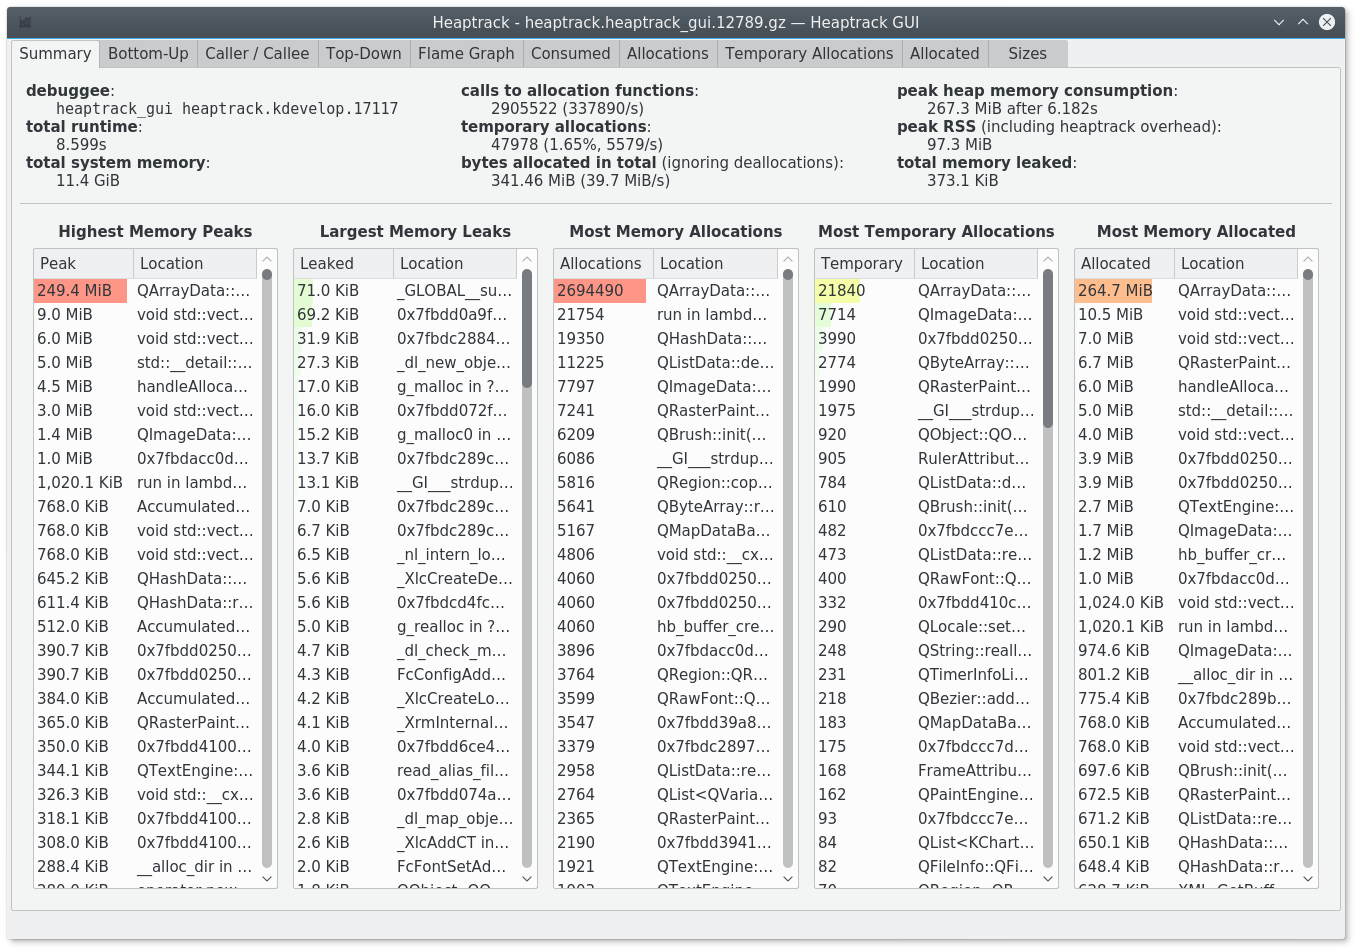
\includegraphics[height=0.8\textheight]{slides/debugging-application-profiling/heaptrack_gui.png}
  \end{center}
\end{frame}

\begin{frame}{\code{heaptrack_gui} - Flamegraph view}
  \begin{center}
    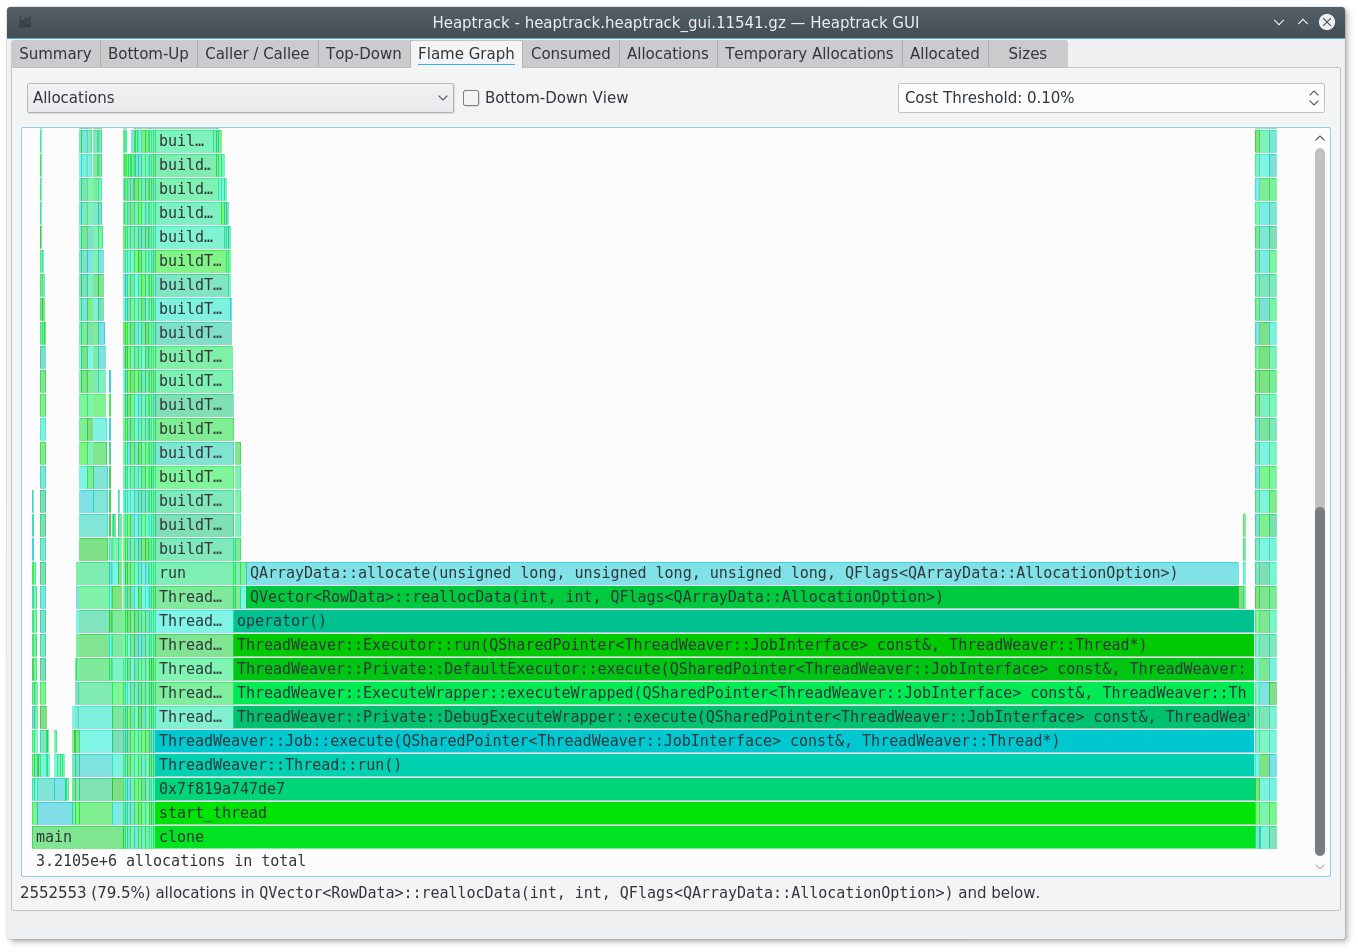
\includegraphics[height=0.8\textheight]{slides/debugging-application-profiling/heaptrack_gui_flamegraph.png}
  \end{center}
\end{frame}

\begin{frame}[fragile]
  \frametitle{memusage}
  \begin{columns}[T]
    \column{0.7\textwidth}
    \begin{itemize}
      \item memusage is a program that leverages \code{libmemusage.so} to profile
            memory usage (\manpage{memusage}{1}) (user-space only).
      \item Can profile heap, stack and also mmap memory usage.
      \item Profiling is output on the console or a PNG file can be generated
            but can also output data to a a binary file for post-treatment by
            other tools.
      \item Lightweight solution compared to valgrind {\em Massif} tool since it
            uses \code{LD_PRELOAD} mechanism.
    \end{itemize}
    \column{0.3\textwidth}
    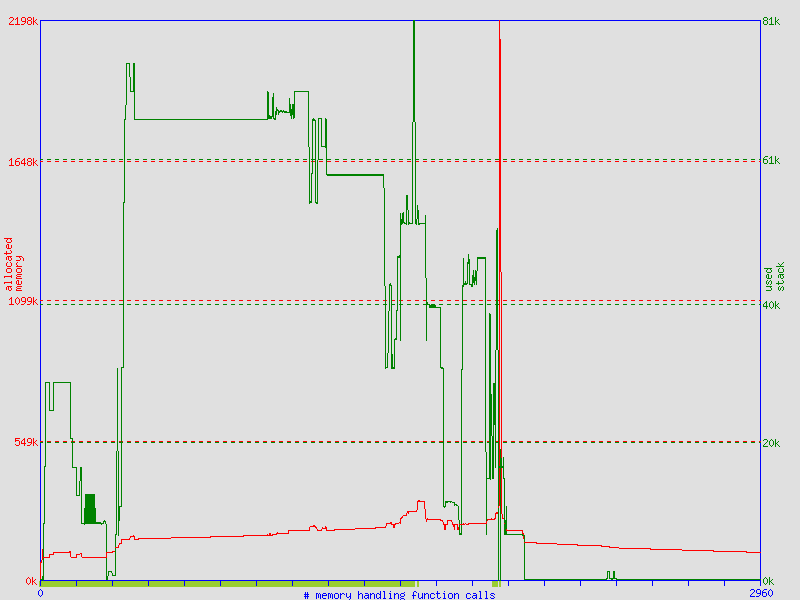
\includegraphics[width=\textwidth]{../slides/debugging-application-profiling/memusage.png}
  \end{columns}
\end{frame}

\begin{frame}[fragile]
  \frametitle{memusage usage}
  \begin{block}{}
    \begin{minted}[fontsize=\tiny]{console}
$ memusage convert foo.png foo.jpg
Memory usage summary: heap total: 2635857, heap peak: 2250856, stack peak: 83696
         total calls   total memory   failed calls
 malloc|       1496        2623648              0
realloc|          6           3744              0  (nomove:0, dec:0, free:0)
 calloc|         16           8465              0
   free|       1480        2521334
Histogram for block sizes:
    0-15            329  21% ==================================================
   16-31            239  15% ====================================
   32-47            287  18% ===========================================
   48-63            321  21% ================================================
   64-79             43   2% ======
   80-95            141   9% =====================
  ...
21424-21439           1  <1% 
32768-32783           1  <1% 
32816-32831           1  <1% 
   large              3  <1% 
    \end{minted}
  \end{block}
\end{frame}

\begin{frame}
  \frametitle{Execution profiling}
  \begin{itemize}
    \item In order to optimize a program, one may have to understand what
          hardware resources are used.
    \item Many hardware elements can have an impact on the program execution:
    \begin{itemize}
      \item Cache performances can be degraded by an application without memory
            spatial locality.
      \item Page miss due to using too much memory without spatial locality.
      \item Alignment faults when doing misaligned accesses.
    \end{itemize}
  \end{itemize}
\end{frame}

\begin{frame}[fragile]
  \frametitle{Using {\em perf stat}}
  \begin{itemize}
    \item \code{perf stat} allows to profile an application by gathering
          performance counters.
    \begin{itemize}
      \item Using performance counters might require {\em root} permissions. This can be
            modified using \code{# echo -1 > /proc/sys/kernel/perf_event_paranoid}
    \end{itemize}
    \item The number of performance counters that are present on the hardware are often
          limited.
    \item Requesting more events than possible will result in multiplexing and
          perf will scale the results.
    \item Collected performance counters result are then approximate.
    \begin{itemize}
      \item To acquire more precise numbers, reduce the number of events that
            observed and run your measure multiple times with other events.
      \item See \url{https://perf.wiki.kernel.org/index.php/Tutorial#multiple_events}{perf wiki}
            for more informations.
    \end{itemize}
  \end{itemize}
\end{frame}

\begin{frame}[fragile]
  \frametitle{{\em perf stat} example (1/2)}
  \begin{block}{}
    \begin{minted}[fontsize=\tiny]{console}
$ perf stat convert foo.png foo.jpg

Performance counter stats for 'convert slides/debugging-kernel-debugging/oops_1.png foo.jpg':

           45,52 msec task-clock                #    1,333 CPUs utilized          
               4      context-switches          #   87,874 /sec                   
               0      cpu-migrations            #    0,000 /sec                   
           1 672      page-faults               #   36,731 K/sec                  
     146 154 800      cycles                    #    3,211 GHz                      (81,16%)
       6 984 741      stalled-cycles-frontend   #    4,78% frontend cycles idle     (91,21%)
      81 002 469      stalled-cycles-backend    #   55,42% backend cycles idle      (91,36%)
     222 687 505      instructions              #    1,52  insn per cycle         
                                                #    0,36  stalled cycles per insn  (91,21%)
      37 776 174      branches                  #  829,884 M/sec                    (74,51%)
         567 408      branch-misses             #    1,50% of all branches          (70,62%)

     0,034156819 seconds time elapsed

     0,041509000 seconds user
     0,004612000 seconds sys
    \end{minted}
  \end{block}
  \begin{itemize}
    \item {\em NOTE: the percentage displayed at the end denotes the time
          during which the kernel measured the event due to multiplexing}
  \end{itemize}
\end{frame}

\begin{frame}[fragile]
  \frametitle{{\em perf stat} example (2/2)}
  \begin{itemize}
    \item List all events:
  \end{itemize}
  \begin{block}{}
    \begin{minted}[fontsize=\tiny]{console}
$ perf list
  List of pre-defined events (to be used in -e):

  branch-instructions OR branches                    [Hardware event]
  branch-misses                                      [Hardware event]
  cache-misses                                       [Hardware event]
  cache-references                                   [Hardware event]
  ...
    \end{minted}
  \end{block}
  \begin{itemize}
    \item Count {\em L1-dcache-load-misses} and {\em branch-load-misses} events for a
          specific command
  \end{itemize}
  \begin{block}{}
    \begin{minted}[fontsize=\tiny]{console}
$ perf stat -e L1-dcache-load-misses,branch-load-misses cat /etc/fstab
...
Performance counter stats for 'cat /etc/fstab':

23 418      L1-dcache-load-misses
 7 192      branch-load-misses
...
    \end{minted}
  \end{block}
\end{frame}

\begin{frame}[fragile]
  \frametitle{{\em Cachegrind}}
  \begin{itemize}
    \item This tools provided by valgrind allows to profile program interactions
          with the instruction and data cache hierarchy.
    \begin{itemize}
      \item {\em Cachegrind} also profiles branch prediction success.
    \end{itemize}
    \item Simulate a machine with independent \code{I$} and \code{D$} backed
          with a unified L2 cache.
    \item Really helpful to profile detect cache usage problems (Too much misses, etc).
  \end{itemize}
  \begin{block}{}
    \begin{minted}[fontsize=\small]{console}
$ valgrind --tool=cachegrind ./my_program
    \end{minted}
  \end{block}
  \begin{itemize}
    \item \code{cg_annotate} is a CLI tool used to visualize cachegrind
          simulation results.
    \item Two simulation results can be diffed using the \code{cg_diff} tool.
  \end{itemize}
\end{frame}

\begin{frame}{Kcachegrind - Visualizing Cachegrind profiling data}
  \begin{center}
    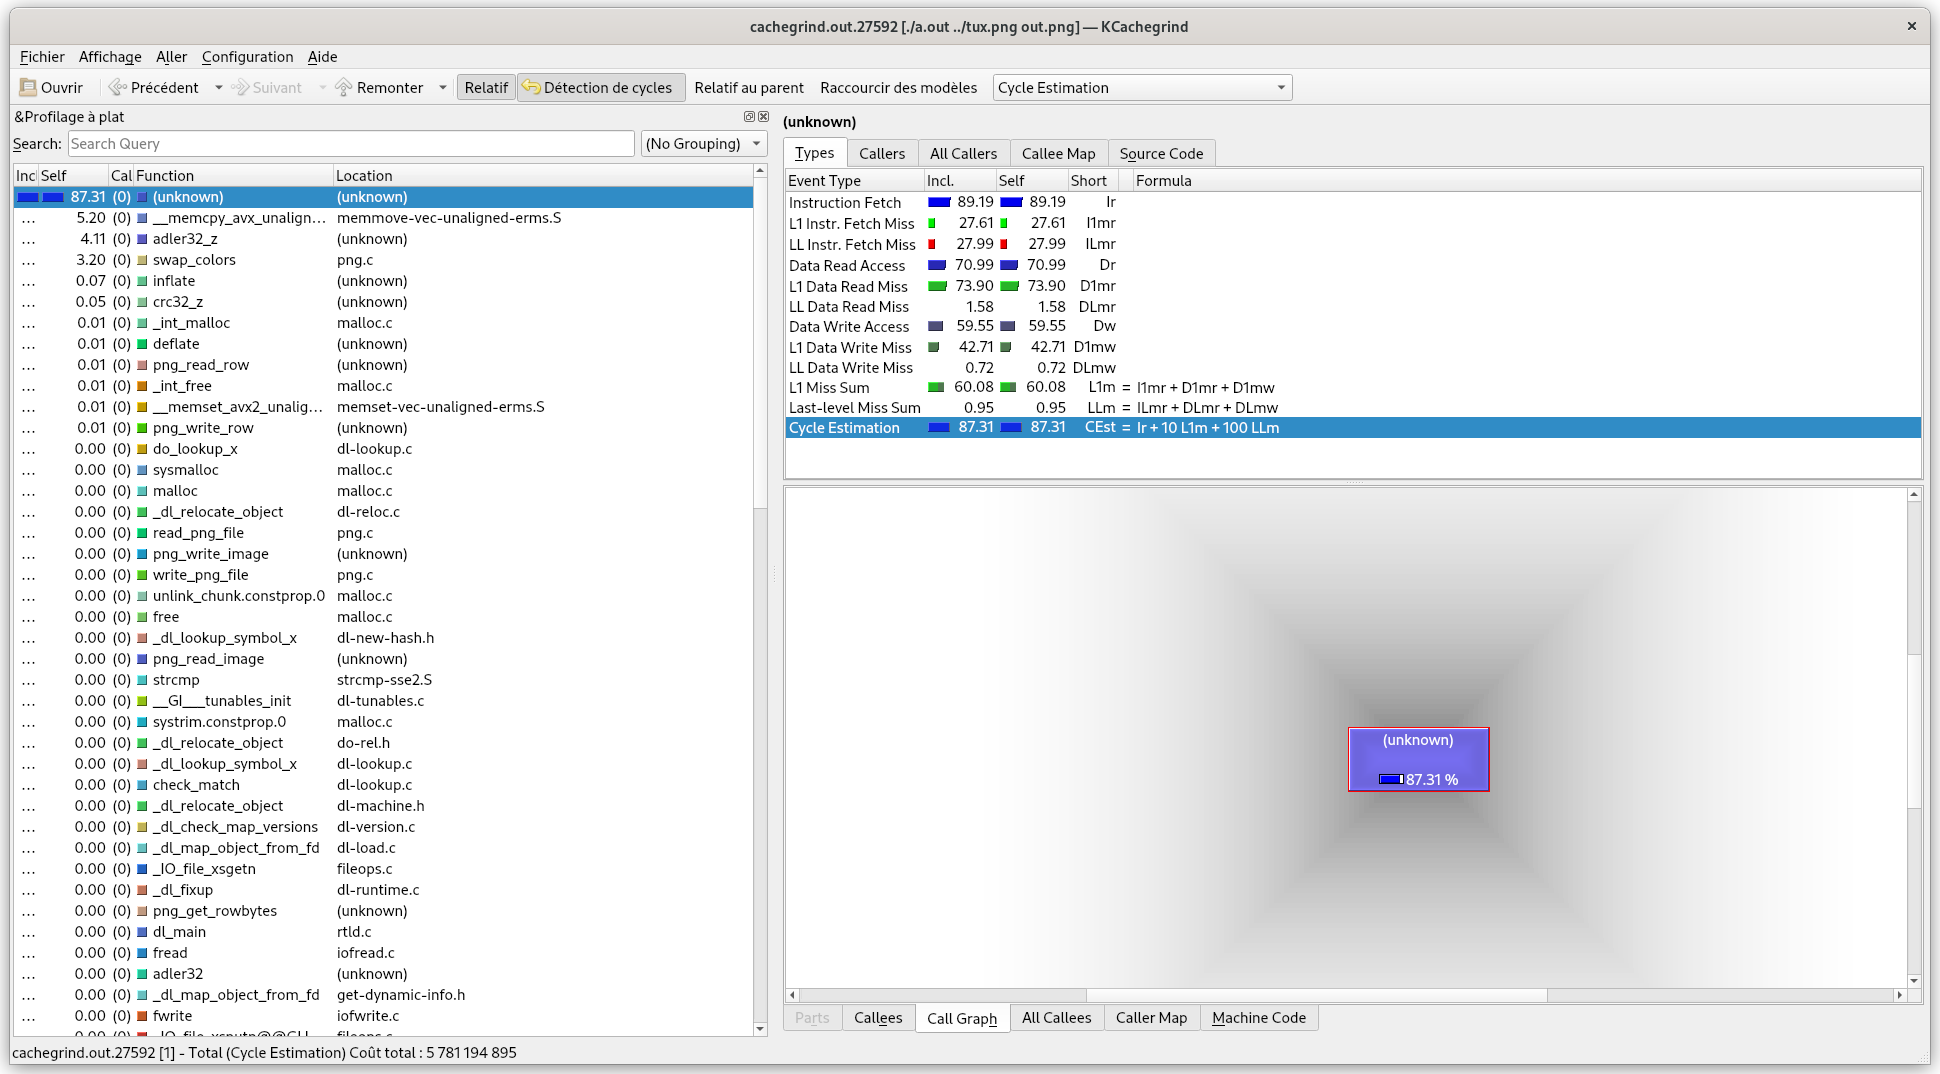
\includegraphics[height=0.8\textheight]{slides/debugging-application-profiling/kcachegrind_cachegrind.png}
  \end{center}
\end{frame}

\begin{frame}[fragile]
  \frametitle{{\em Callgrind}}
  \begin{itemize}
    \item Provided by valgrind and allows to profile an application call graph
          (user-space only).
    \item Collects the number of instructions executed during your program
          execution and associate these data with the source lines
    \item Record the call relationship between functions and their call
          count.
  \begin{block}{}
    \begin{minted}[fontsize=\small]{console}
$ valgrind --tool=callgrind ./my_program
    \end{minted}
  \end{block}

  \item \code{callgrind_annotate} is a CLI tool used to visualize callgrind
        simulation results.
  \item Results can also be visualized using a GUI tool named Kcachegrind.
  \item The cache simulation (done using cachegrind) has some accuracy
        shortcomings (See \href{https://valgrind.org/docs/manual/cg-manual.html#cg-manual.annopts.accuracy}{Cachegrind accuracy})
  \end{itemize}
\end{frame}

\begin{frame}{Kcachegrind - Visualizing Callgrind profiling data}
  \begin{center}
    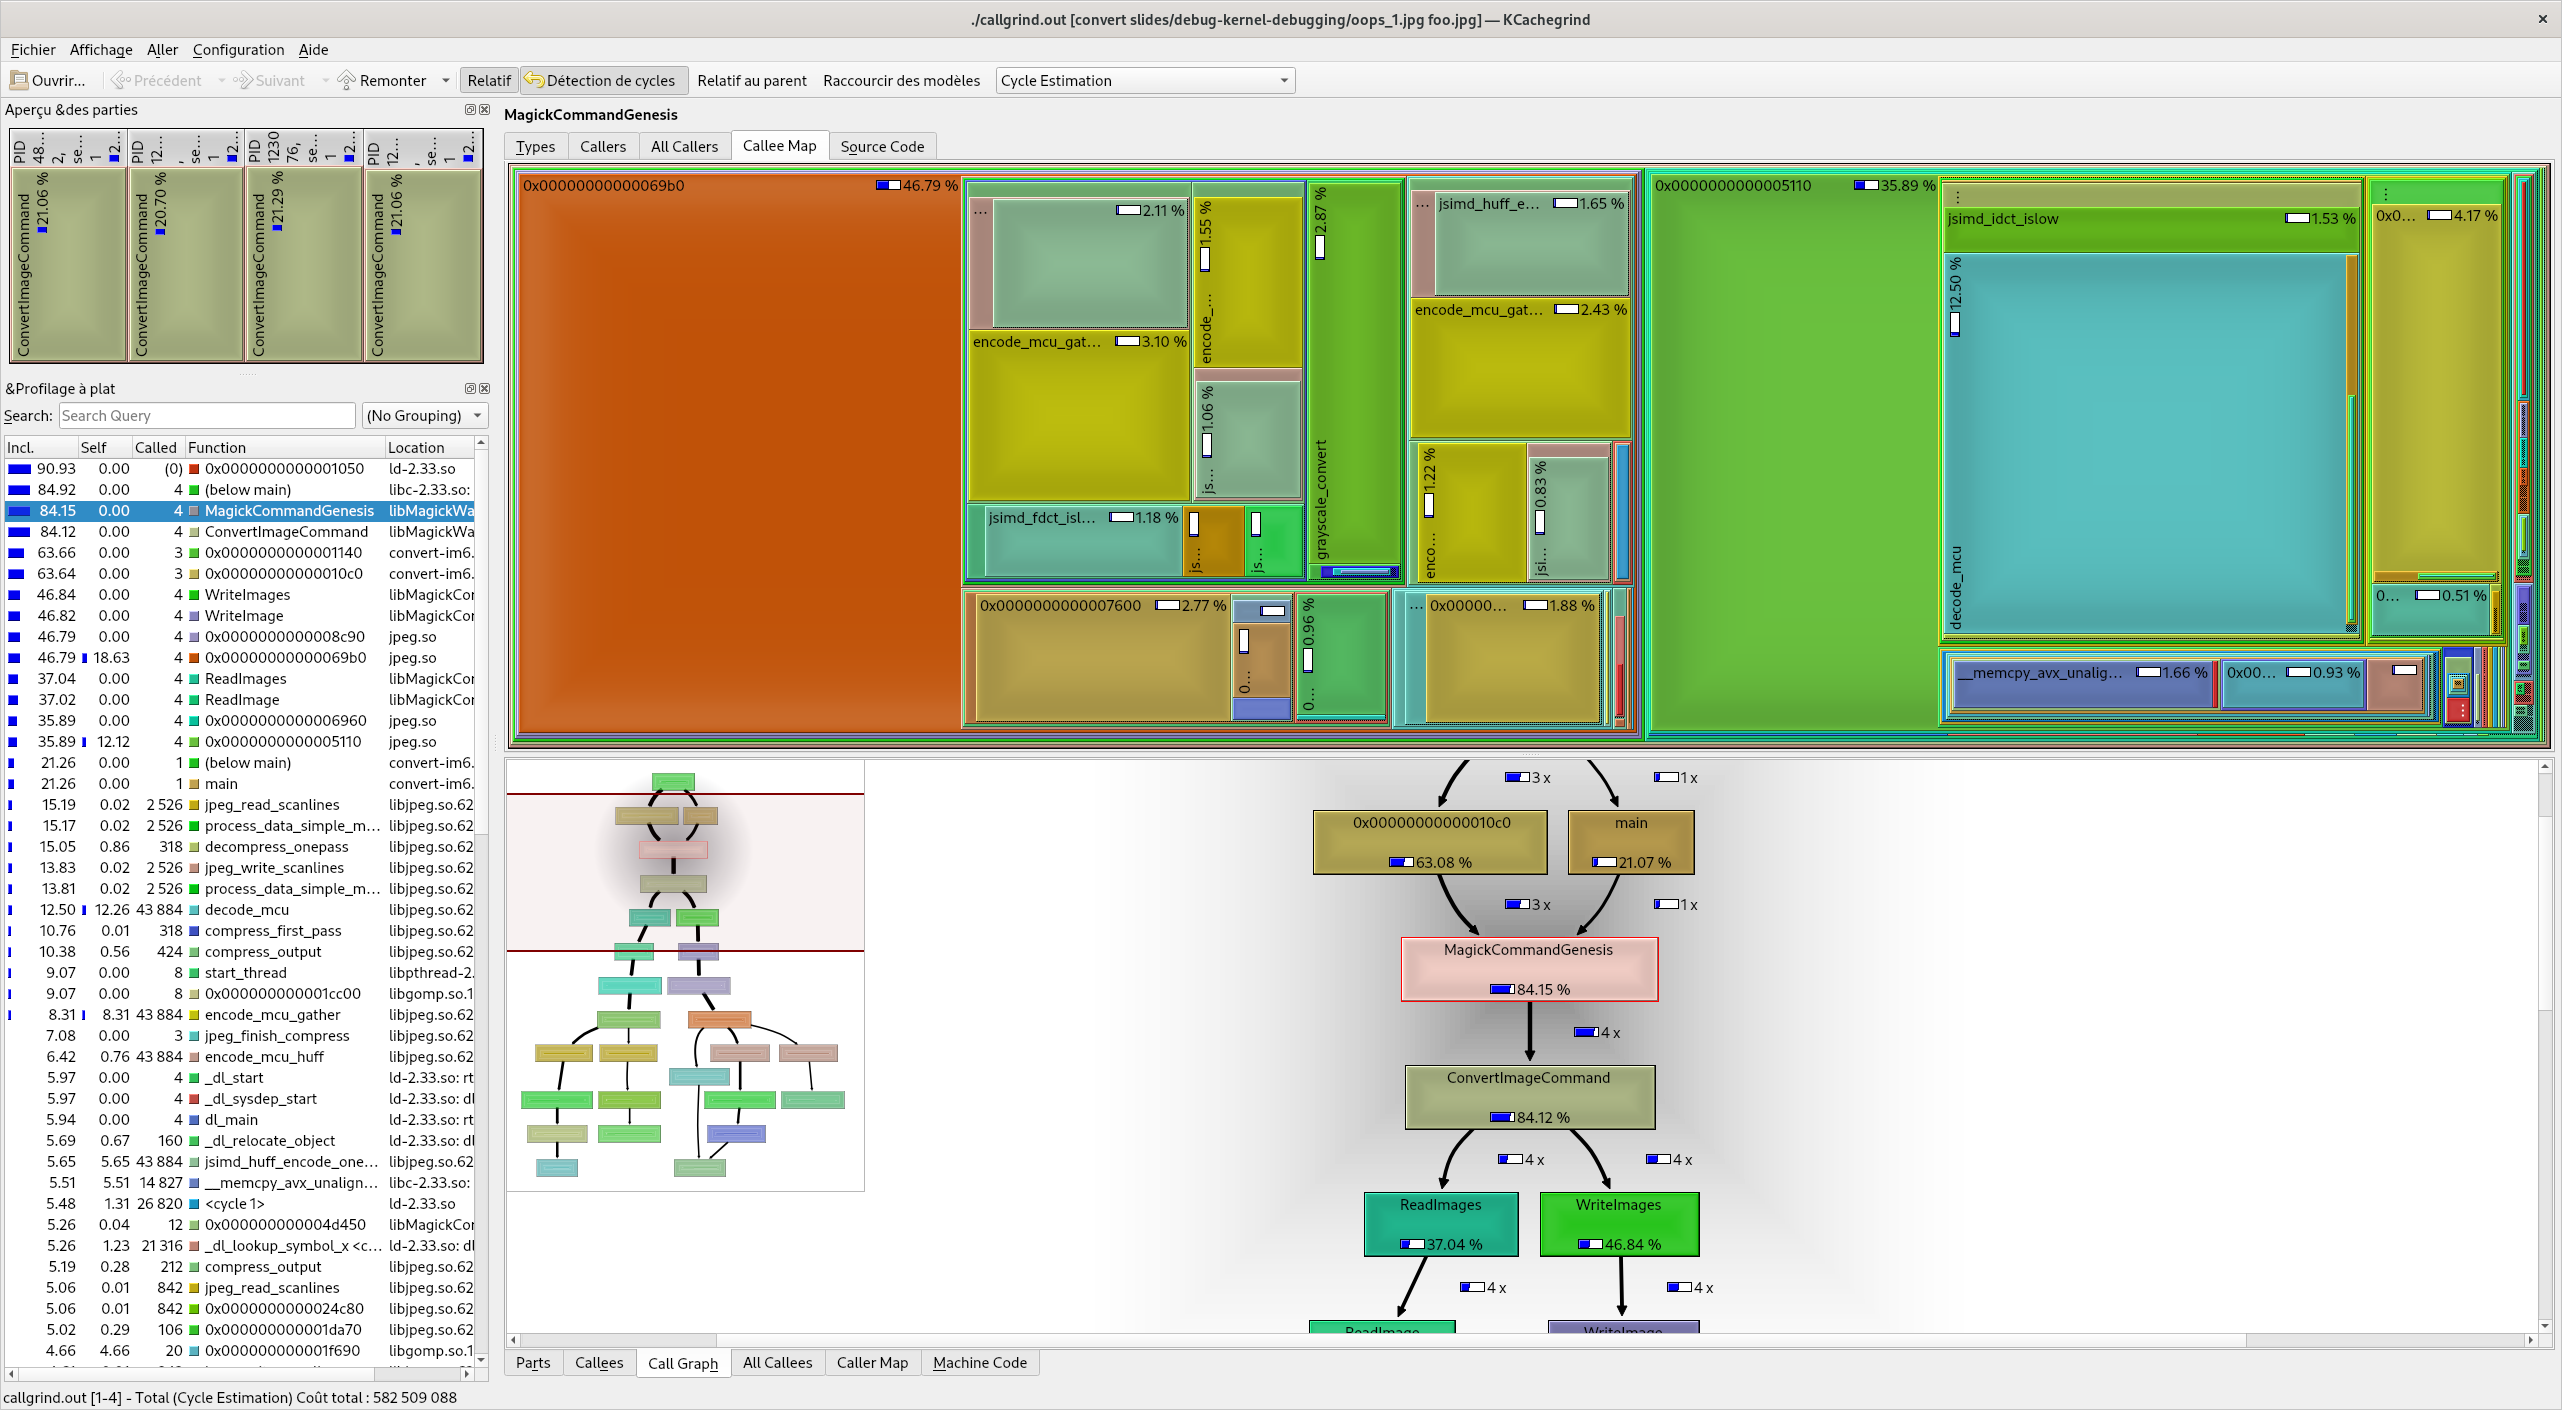
\includegraphics[height=0.8\textheight]{slides/debugging-application-profiling/kcachegrind_callgrind.png}
  \end{center}
\end{frame}
